\documentclass{article}\usepackage[]{graphicx}\usepackage[]{color}
%% maxwidth is the original width if it is less than linewidth
%% otherwise use linewidth (to make sure the graphics do not exceed the margin)
\makeatletter
\def\maxwidth{ %
  \ifdim\Gin@nat@width>\linewidth
    \linewidth
  \else
    \Gin@nat@width
  \fi
}
\makeatother

\definecolor{fgcolor}{rgb}{0.345, 0.345, 0.345}
\newcommand{\hlnum}[1]{\textcolor[rgb]{0.686,0.059,0.569}{#1}}%
\newcommand{\hlstr}[1]{\textcolor[rgb]{0.192,0.494,0.8}{#1}}%
\newcommand{\hlcom}[1]{\textcolor[rgb]{0.678,0.584,0.686}{\textit{#1}}}%
\newcommand{\hlopt}[1]{\textcolor[rgb]{0,0,0}{#1}}%
\newcommand{\hlstd}[1]{\textcolor[rgb]{0.345,0.345,0.345}{#1}}%
\newcommand{\hlkwa}[1]{\textcolor[rgb]{0.161,0.373,0.58}{\textbf{#1}}}%
\newcommand{\hlkwb}[1]{\textcolor[rgb]{0.69,0.353,0.396}{#1}}%
\newcommand{\hlkwc}[1]{\textcolor[rgb]{0.333,0.667,0.333}{#1}}%
\newcommand{\hlkwd}[1]{\textcolor[rgb]{0.737,0.353,0.396}{\textbf{#1}}}%

\usepackage{framed}
\makeatletter
\newenvironment{kframe}{%
 \def\at@end@of@kframe{}%
 \ifinner\ifhmode%
  \def\at@end@of@kframe{\end{minipage}}%
  \begin{minipage}{\columnwidth}%
 \fi\fi%
 \def\FrameCommand##1{\hskip\@totalleftmargin \hskip-\fboxsep
 \colorbox{shadecolor}{##1}\hskip-\fboxsep
     % There is no \\@totalrightmargin, so:
     \hskip-\linewidth \hskip-\@totalleftmargin \hskip\columnwidth}%
 \MakeFramed {\advance\hsize-\width
   \@totalleftmargin\z@ \linewidth\hsize
   \@setminipage}}%
 {\par\unskip\endMakeFramed%
 \at@end@of@kframe}
\makeatother

\definecolor{shadecolor}{rgb}{.97, .97, .97}
\definecolor{messagecolor}{rgb}{0, 0, 0}
\definecolor{warningcolor}{rgb}{1, 0, 1}
\definecolor{errorcolor}{rgb}{1, 0, 0}
\newenvironment{knitrout}{}{} % an empty environment to be redefined in TeX

\usepackage{alltt}
\IfFileExists{upquote.sty}{\usepackage{upquote}}{}
\begin{document}

\begin{knitrout}
\definecolor{shadecolor}{rgb}{0.969, 0.969, 0.969}\color{fgcolor}\begin{kframe}
\begin{alltt}
\hlcom{#ROXANA BEATRIZ RONQUILLO UMA�A}

\hlcom{#CARTOGRAFIA EN R}
\end{alltt}
\end{kframe}
\end{knitrout}

\begin{knitrout}
\definecolor{shadecolor}{rgb}{0.969, 0.969, 0.969}\color{fgcolor}\begin{kframe}
\begin{alltt}
\hlcom{#EJEMPLO 1: Se representa con un punto rojo la capital de Francia.}

\hlcom{#Cargamos la librer�a}
\hlkwd{library}\hlstd{(maptools)}
\end{alltt}


{\ttfamily\noindent\color{warningcolor}{\#\# Warning: package 'maptools' was built under R version 3.2.2}}

{\ttfamily\noindent\itshape\color{messagecolor}{\#\# Loading required package: sp}}

{\ttfamily\noindent\color{warningcolor}{\#\# Warning: package 'sp' was built under R version 3.2.2}}

{\ttfamily\noindent\itshape\color{messagecolor}{\#\# Checking rgeos availability: FALSE\\\#\#\ \ 	Note: when rgeos is not available, polygon geometry 	computations in maptools depend on gpclib,\\\#\#\ \ 	which has a restricted licence. It is disabled by default;\\\#\#\ \ 	to enable gpclib, type gpclibPermit()}}\begin{alltt}
\hlcom{#Se cargan los datos obtenidos de www.gadm.org}
\hlstd{france}\hlkwb{<-}\hlkwd{readShapeSpatial}\hlstd{(}\hlstr{"FRA_adm0.shp"}\hlstd{,}\hlkwc{proj4string}\hlstd{=}\hlkwd{CRS}\hlstd{(}\hlstr{"+proj=longlat"}\hlstd{))}
\hlcom{#mostramos el grafico}
\hlkwd{plot}\hlstd{(france)}
\end{alltt}
\end{kframe}
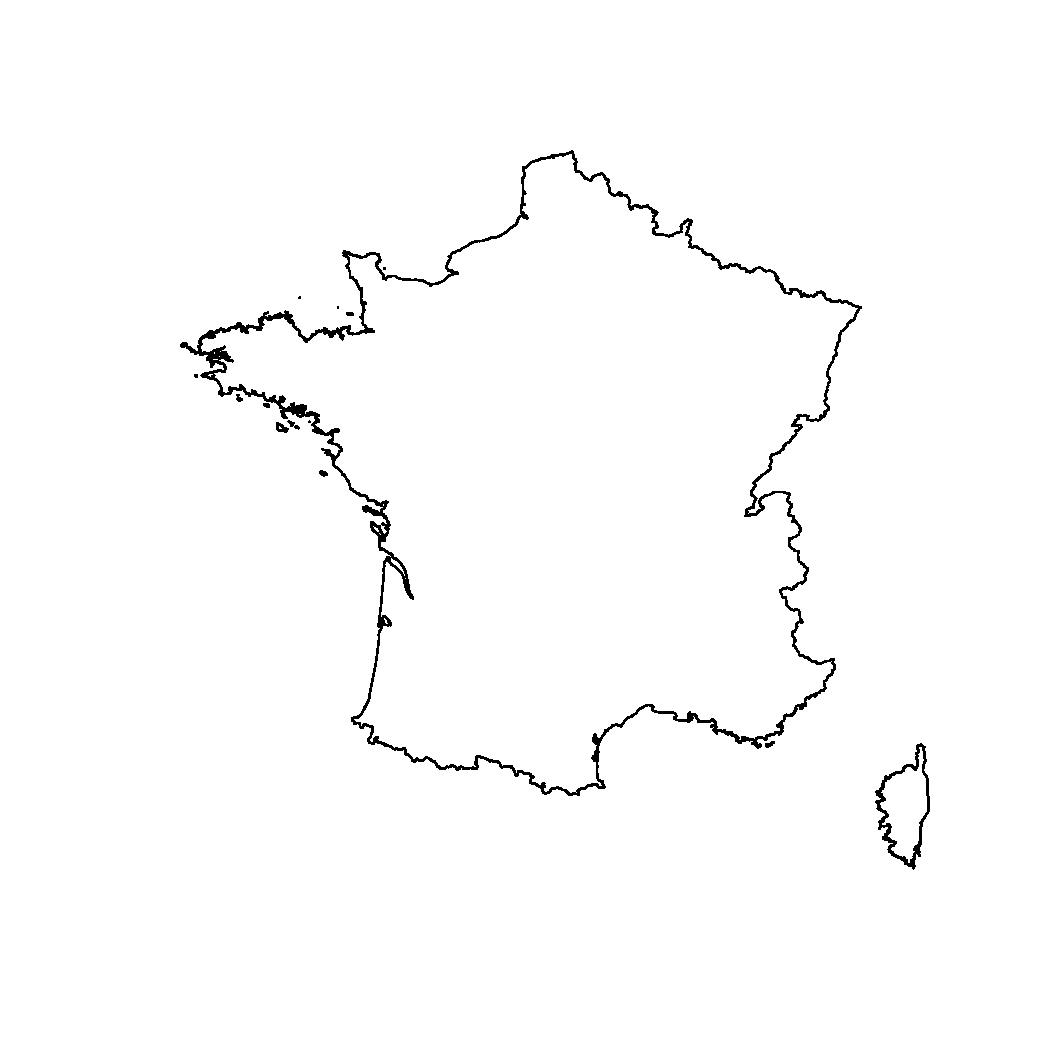
\includegraphics[width=\maxwidth]{figure/unnamed-chunk-2-1} 
\begin{kframe}\begin{alltt}
\hlcom{#Se grafica el punto correspondiente a la capital de Francia (Paris)}
\hlkwd{plot}\hlstd{(france,}\hlkwc{xlim}\hlstd{=}\hlkwd{c}\hlstd{(}\hlnum{1}\hlstd{,}\hlnum{4}\hlstd{),}\hlkwc{ylim}\hlstd{=}\hlkwd{c}\hlstd{(}\hlnum{41.5}\hlstd{,}\hlnum{51}\hlstd{))}
\hlkwd{points}\hlstd{(}\hlnum{2.349}\hlstd{,}\hlnum{48.853}\hlstd{,}\hlkwc{pch}\hlstd{=}\hlnum{20}\hlstd{,}\hlkwc{col}\hlstd{=}\hlstr{"red"}\hlstd{,}\hlkwc{cex}\hlstd{=}\hlnum{2}\hlstd{)}
\end{alltt}
\end{kframe}
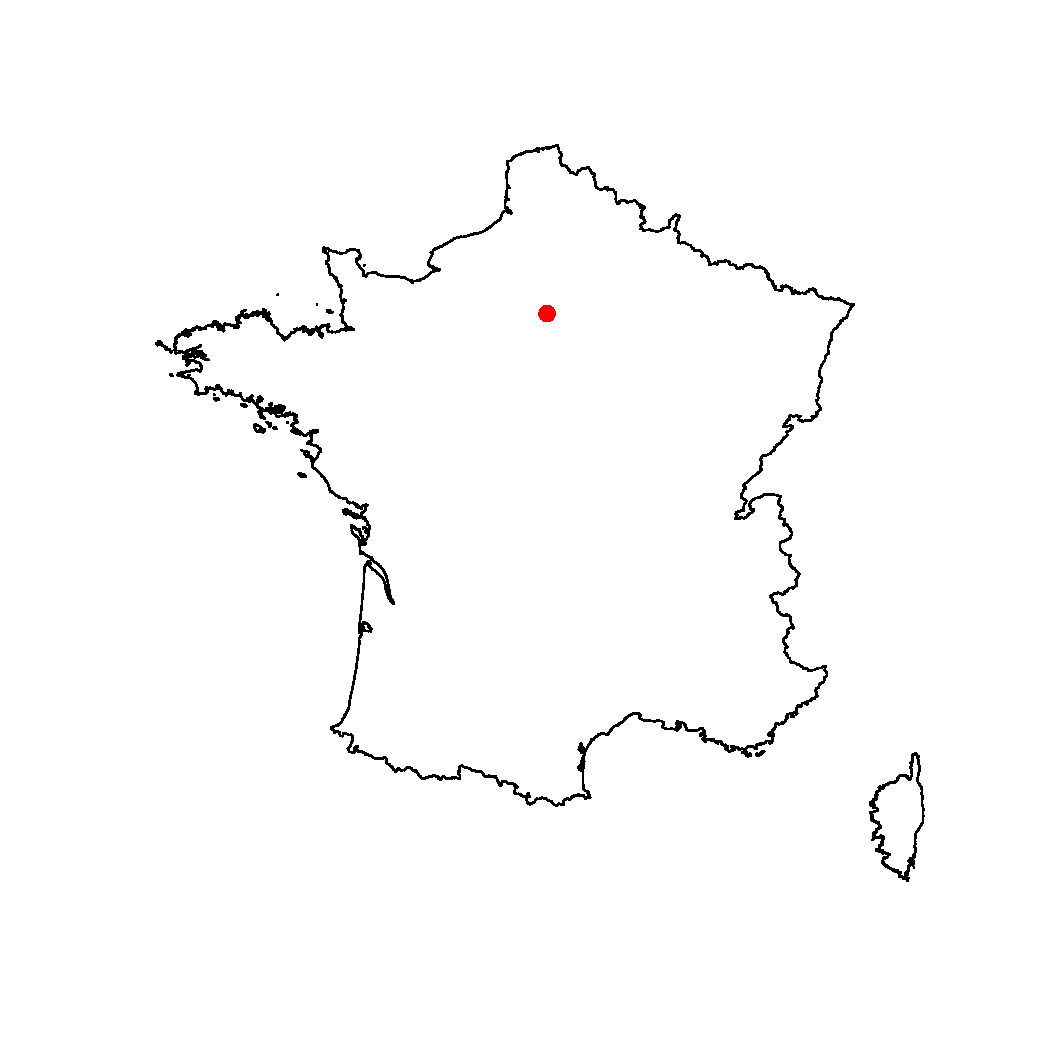
\includegraphics[width=\maxwidth]{figure/unnamed-chunk-2-2} 

\end{knitrout}

\begin{knitrout}
\definecolor{shadecolor}{rgb}{0.969, 0.969, 0.969}\color{fgcolor}\begin{kframe}
\begin{alltt}
\hlcom{#EJEMPLO 2: Zona de los andes.}

\hlcom{# cargamos libreria}
\hlkwd{library}\hlstd{(}\hlstr{"XML"}\hlstd{)}
\end{alltt}


{\ttfamily\noindent\color{warningcolor}{\#\# Warning: package 'XML' was built under R version 3.2.2}}\begin{alltt}
\hlcom{# primer data frame}
\hlstd{theurl} \hlkwb{<-} \hlstr{"http://www.peaklist.org/WWlists/ultras/andes1.html"}
\hlstd{tables} \hlkwb{<-} \hlkwd{readHTMLTable}\hlstd{(theurl)}
\hlstd{n.rows} \hlkwb{<-} \hlkwd{unlist}\hlstd{(}\hlkwd{lapply}\hlstd{(tables,} \hlkwa{function}\hlstd{(}\hlkwc{t}\hlstd{)} \hlkwd{dim}\hlstd{(t)[}\hlnum{1}\hlstd{]))}
\hlstd{df}\hlkwb{<-}\hlstd{tables[[}\hlkwd{which.max}\hlstd{(n.rows)]]}
\hlstd{df}\hlkwb{<-}\hlstd{df[}\hlnum{3}\hlopt{:}\hlkwd{nrow}\hlstd{(df),}\hlkwd{c}\hlstd{(}\hlnum{2}\hlstd{,}\hlnum{3}\hlstd{,}\hlnum{4}\hlstd{,}\hlnum{7}\hlstd{,}\hlnum{8}\hlstd{)]}
\hlkwd{names}\hlstd{(df)}\hlkwb{=}\hlkwd{c}\hlstd{(}\hlstr{"cumbre"}\hlstd{,} \hlstr{"pais"}\hlstd{,} \hlstr{"altura_m"}\hlstd{,} \hlstr{"lat_geo"}\hlstd{,} \hlstr{"lng_geo"}\hlstd{)}
\hlstd{df1}\hlkwb{<-}\hlkwd{na.omit}\hlstd{(df)}
\hlcom{# segundo data frame}
\hlstd{theurl} \hlkwb{<-} \hlstr{"http://www.peaklist.org/WWlists/ultras/andes2.html"}
\hlstd{tables} \hlkwb{<-} \hlkwd{readHTMLTable}\hlstd{(theurl)}
\hlstd{n.rows} \hlkwb{<-} \hlkwd{unlist}\hlstd{(}\hlkwd{lapply}\hlstd{(tables,} \hlkwa{function}\hlstd{(}\hlkwc{t}\hlstd{)} \hlkwd{dim}\hlstd{(t)[}\hlnum{1}\hlstd{]))}
\hlstd{df}\hlkwb{<-}\hlstd{tables[[}\hlkwd{which.max}\hlstd{(n.rows)]]}
\hlstd{df}\hlkwb{<-}\hlstd{df[}\hlnum{3}\hlopt{:}\hlkwd{nrow}\hlstd{(df),}\hlkwd{c}\hlstd{(}\hlnum{2}\hlstd{,}\hlnum{3}\hlstd{,}\hlnum{4}\hlstd{,}\hlnum{7}\hlstd{,}\hlnum{8}\hlstd{)]}
\hlkwd{names}\hlstd{(df)}\hlkwb{=}\hlkwd{c}\hlstd{(}\hlstr{"cumbre"}\hlstd{,} \hlstr{"pais"}\hlstd{,} \hlstr{"altura_m"}\hlstd{,} \hlstr{"lat_geo"}\hlstd{,} \hlstr{"lng_geo"}\hlstd{)}
\hlstd{df2}\hlkwb{<-}\hlkwd{na.omit}\hlstd{(df)}

\hlcom{# tercer data frame}
\hlstd{theurl} \hlkwb{<-} \hlstr{"http://www.peaklist.org/WWlists/ultras/andes3.html"}
\hlstd{tables} \hlkwb{<-} \hlkwd{readHTMLTable}\hlstd{(theurl)}
\hlstd{n.rows} \hlkwb{<-} \hlkwd{unlist}\hlstd{(}\hlkwd{lapply}\hlstd{(tables,} \hlkwa{function}\hlstd{(}\hlkwc{t}\hlstd{)} \hlkwd{dim}\hlstd{(t)[}\hlnum{1}\hlstd{]))}
\hlstd{df}\hlkwb{<-}\hlstd{tables[[}\hlkwd{which.max}\hlstd{(n.rows)]]}
\hlstd{df}\hlkwb{<-}\hlstd{df[}\hlnum{3}\hlopt{:}\hlkwd{nrow}\hlstd{(df),}\hlkwd{c}\hlstd{(}\hlnum{2}\hlstd{,}\hlnum{3}\hlstd{,}\hlnum{4}\hlstd{,}\hlnum{7}\hlstd{,}\hlnum{8}\hlstd{)]}
\hlkwd{names}\hlstd{(df)}\hlkwb{=}\hlkwd{c}\hlstd{(}\hlstr{"cumbre"}\hlstd{,} \hlstr{"pais"}\hlstd{,} \hlstr{"altura_m"}\hlstd{,} \hlstr{"lat_geo"}\hlstd{,} \hlstr{"lng_geo"}\hlstd{)}
\hlstd{df3}\hlkwb{<-}\hlkwd{na.omit}\hlstd{(df)}

\hlcom{# unimos los tres data frame en uno y convertimos las columnas de altura a entero y las coordenadas a texto}
\hlstd{df}\hlkwb{<-}\hlkwd{rbind}\hlstd{(df1,df2,df3)}
\hlstd{df}\hlopt{$}\hlstd{altura_m}\hlkwb{<-}\hlkwd{as.integer}\hlstd{(}\hlkwd{as.character}\hlstd{(df}\hlopt{$}\hlstd{altura_m))}
\hlstd{df}\hlopt{$}\hlstd{lat_geo}\hlkwb{<-}\hlkwd{as.character}\hlstd{(df}\hlopt{$}\hlstd{lat_geo)}
\hlstd{df}\hlopt{$}\hlstd{lng_geo}\hlkwb{<-}\hlkwd{as.character}\hlstd{(df}\hlopt{$}\hlstd{lng_geo)}

\hlcom{# creamos esta funci�n para transformar las coordenadas geogr�ficas a decimal}
\hlstd{geo2dec}\hlkwb{<-}\hlkwa{function}\hlstd{(}\hlkwc{c}\hlstd{) \{}
  \hlstd{z}\hlkwb{<-}\hlkwd{sapply}\hlstd{(} \hlkwd{strsplit}\hlstd{(c,} \hlstr{"[º\textbackslash{}'\textbackslash{}"]"}\hlstd{), as.character )}
  \hlstd{dec}\hlkwb{<-} \hlkwd{as.numeric}\hlstd{(z[}\hlnum{1}\hlstd{, ])} \hlopt{+} \hlkwd{as.numeric}\hlstd{(z[}\hlnum{3}\hlstd{, ])}\hlopt{/}\hlnum{60} \hlopt{+} \hlkwd{as.numeric}\hlstd{(z[}\hlnum{4}\hlstd{, ])}\hlopt{/}\hlnum{3600}
  \hlkwa{if} \hlstd{(z[}\hlnum{1}\hlstd{, ]}\hlopt{==}\hlstr{"N"}\hlopt{||}\hlstd{z[}\hlnum{1}\hlstd{, ]}\hlopt{==}\hlstr{"E"}\hlstd{) dec} \hlkwa{else} \hlopt{-}\hlstd{dec}
\hlstd{\}}

\hlcom{# agregamos dos columnas con la latitud y longitud en coordenadas decimales}
\hlstd{df}\hlopt{$}\hlstd{latitude}\hlkwb{<-}\hlkwd{geo2dec}\hlstd{(df}\hlopt{$}\hlstd{lat_geo)}
\hlstd{df}\hlopt{$}\hlstd{longitude}\hlkwb{<-}\hlkwd{geo2dec}\hlstd{(df}\hlopt{$}\hlstd{lng_geo)}

\hlcom{# cargamos libreria}
\hlkwd{library}\hlstd{(}\hlstr{"ggmap"}\hlstd{)}
\end{alltt}


{\ttfamily\noindent\color{warningcolor}{\#\# Warning: package 'ggmap' was built under R version 3.2.2}}

{\ttfamily\noindent\itshape\color{messagecolor}{\#\# Loading required package: ggplot2}}

{\ttfamily\noindent\color{warningcolor}{\#\# Warning: package 'ggplot2' was built under R version 3.2.2}}\begin{alltt}
\hlcom{# descargamos el mapa de Chile desde Google}
\hlstd{map} \hlkwb{<-} \hlkwd{get_map}\hlstd{(}\hlkwc{location} \hlstd{=} \hlstr{'Chile'}\hlstd{,} \hlkwc{zoom} \hlstd{=} \hlnum{4}\hlstd{,} \hlkwc{maptype} \hlstd{=} \hlstr{"terrain"}\hlstd{)}
\end{alltt}


{\ttfamily\noindent\itshape\color{messagecolor}{\#\# Map from URL : http://maps.googleapis.com/maps/api/staticmap?center=Chile\&zoom=4\&size=640x640\&scale=2\&maptype=terrain\&language=en-EN\&sensor=false\\\#\# Information from URL : http://maps.googleapis.com/maps/api/geocode/json?address=Chile\&sensor=false}}\begin{alltt}
\hlcom{# pintamos los puntos de nuestro data frame en el mapa}
\hlstd{andes} \hlkwb{<-} \hlkwd{ggmap}\hlstd{(map)} \hlopt{+} \hlkwd{geom_point}\hlstd{(}\hlkwc{data}\hlstd{=df,} \hlkwd{aes}\hlstd{(}\hlkwc{x}\hlstd{=longitude,} \hlkwc{y}\hlstd{=latitude,} \hlkwc{colour}\hlstd{=altura_m),}\hlkwc{alpha} \hlstd{=} \hlnum{0.6}\hlstd{,} \hlkwc{show_guide} \hlstd{=} \hlnum{FALSE}\hlstd{,} \hlkwc{size}\hlstd{=}\hlnum{4}\hlstd{)}

\hlcom{# agregamos una leyenda y escala coloreada}
\hlstd{andes} \hlkwb{<-} \hlstd{andes} \hlopt{+} \hlkwd{scale_colour_continuous}\hlstd{(}\hlkwc{low} \hlstd{=} \hlstr{"red"}\hlstd{,} \hlkwc{high} \hlstd{=} \hlstr{"blue"}\hlstd{,} \hlkwc{space} \hlstd{=} \hlstr{"Lab"}\hlstd{,} \hlkwc{guide} \hlstd{=} \hlstr{"colorbar"}\hlstd{)}
\hlcom{# generamos el mapa}
\hlstd{andes}
\end{alltt}
\end{kframe}
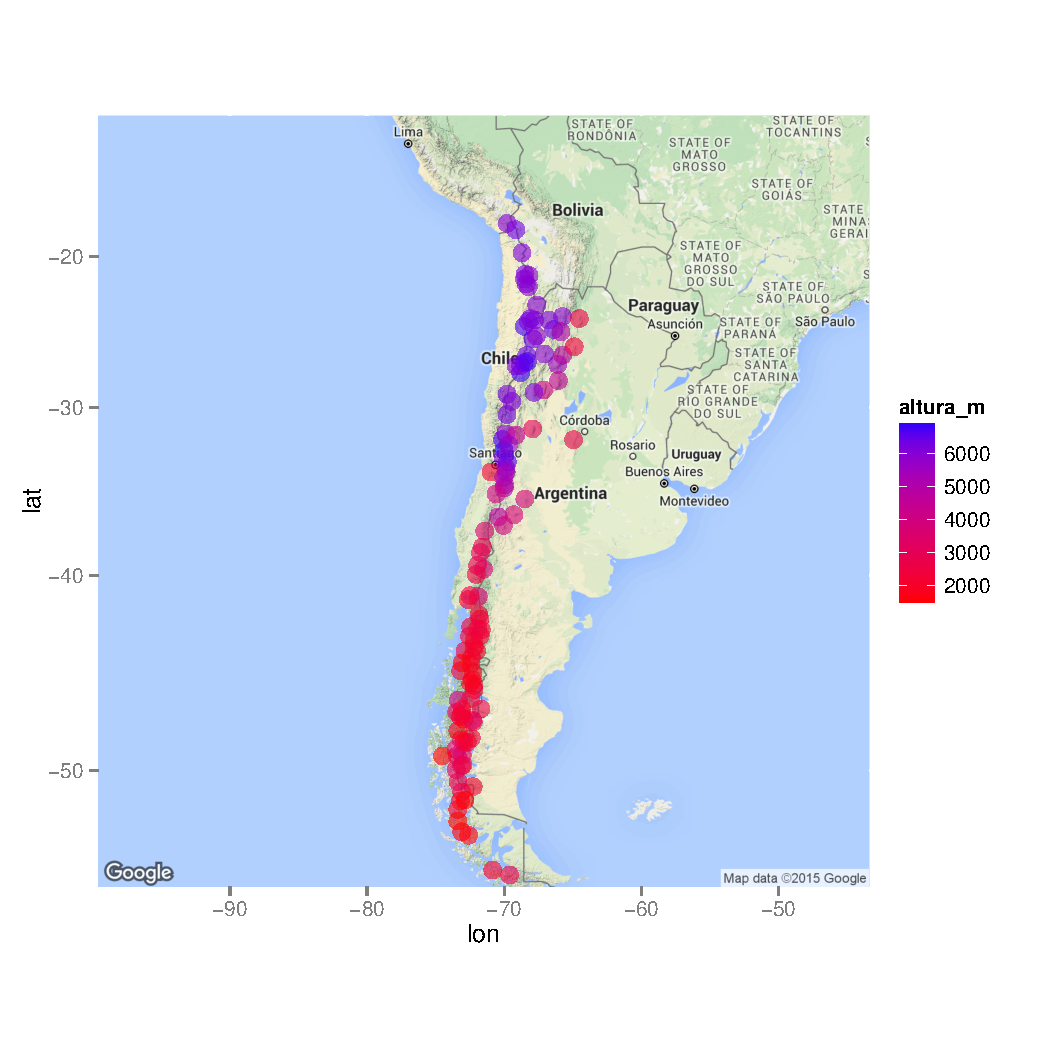
\includegraphics[width=\maxwidth]{figure/unnamed-chunk-3-1} 

\end{knitrout}

\begin{knitrout}
\definecolor{shadecolor}{rgb}{0.969, 0.969, 0.969}\color{fgcolor}\begin{kframe}
\begin{alltt}
\hlcom{#EJEMPLO 3: Provinvias de peru.}

\hlcom{#Se carga la libreria}
\hlkwd{library}\hlstd{(sp)}
\hlcom{#Se descargan los datos de http://gadm.org/country}
\hlstd{peru} \hlkwb{<-} \hlkwd{readRDS}\hlstd{(}\hlstr{"PER_adm2.rds"}\hlstd{)}
\hlkwd{names}\hlstd{(peru)}
\end{alltt}
\begin{verbatim}
##  [1] "OBJECTID"  "ID_0"      "ISO"       "NAME_0"    "ID_1"     
##  [6] "NAME_1"    "ID_2"      "NAME_2"    "HASC_2"    "CCN_2"    
## [11] "CCA_2"     "TYPE_2"    "ENGTYPE_2" "NL_NAME_2" "VARNAME_2"
\end{verbatim}
\begin{alltt}
\hlcom{# El mapa y sus caracter�sticas est�n cargados en gadm por provincias}
\hlstd{mapalima} \hlkwb{<-} \hlstd{peru[peru}\hlopt{@}\hlkwc{data}\hlopt{$}\hlstd{NAME_1} \hlopt{==} \hlstr{"Lima"}\hlstd{,]}
\hlcom{# Seleccionamos solo los datos de la provincias}
\hlstd{datalima} \hlkwb{<-} \hlkwd{data.frame}\hlstd{(mapalima)}
\hlstd{datalima[}\hlnum{7}\hlstd{];mapalima}\hlopt{$}\hlstd{NAME_2;}
\end{alltt}
\begin{verbatim}
##     ID_2
## 129  129
## 130  130
## 131  131
## 132  132
## 133  133
## 134  134
## 135  135
## 136  136
## 137  137
## [1] "Barranca"   "Ca�ete"     "Cajatambo"  "Canta"      "Huaral"    
## [6] "Huarochiri" "Huaura"     "Oyon"       "Yauyos"
\end{verbatim}
\begin{alltt}
\hlcom{#creamos el factor seg�n los nombres de las provincias elegidas}
\hlstd{mapalima}\hlopt{$}\hlstd{provincias} \hlkwb{<-} \hlkwd{factor}\hlstd{(mapalima}\hlopt{$}\hlstd{NAME_2)}
\hlcom{#la funci�n factor es para eliminar los niveles que no existen}
\hlstd{col} \hlkwb{<-} \hlkwd{rainbow}\hlstd{(}\hlkwd{length}\hlstd{(}\hlkwd{levels}\hlstd{(mapalima}\hlopt{$}\hlstd{provincias )))}
\hlcom{# asignamos los colores seg�n los niveles}
\hlcom{# mostramos el mapa}
\hlkwd{spplot}\hlstd{(mapalima,} \hlstr{"provincias"}\hlstd{,} \hlkwc{col.regions} \hlstd{= col,} \hlkwc{main} \hlstd{=} \hlstr{"Lima Provincias"}\hlstd{)}
\end{alltt}
\end{kframe}
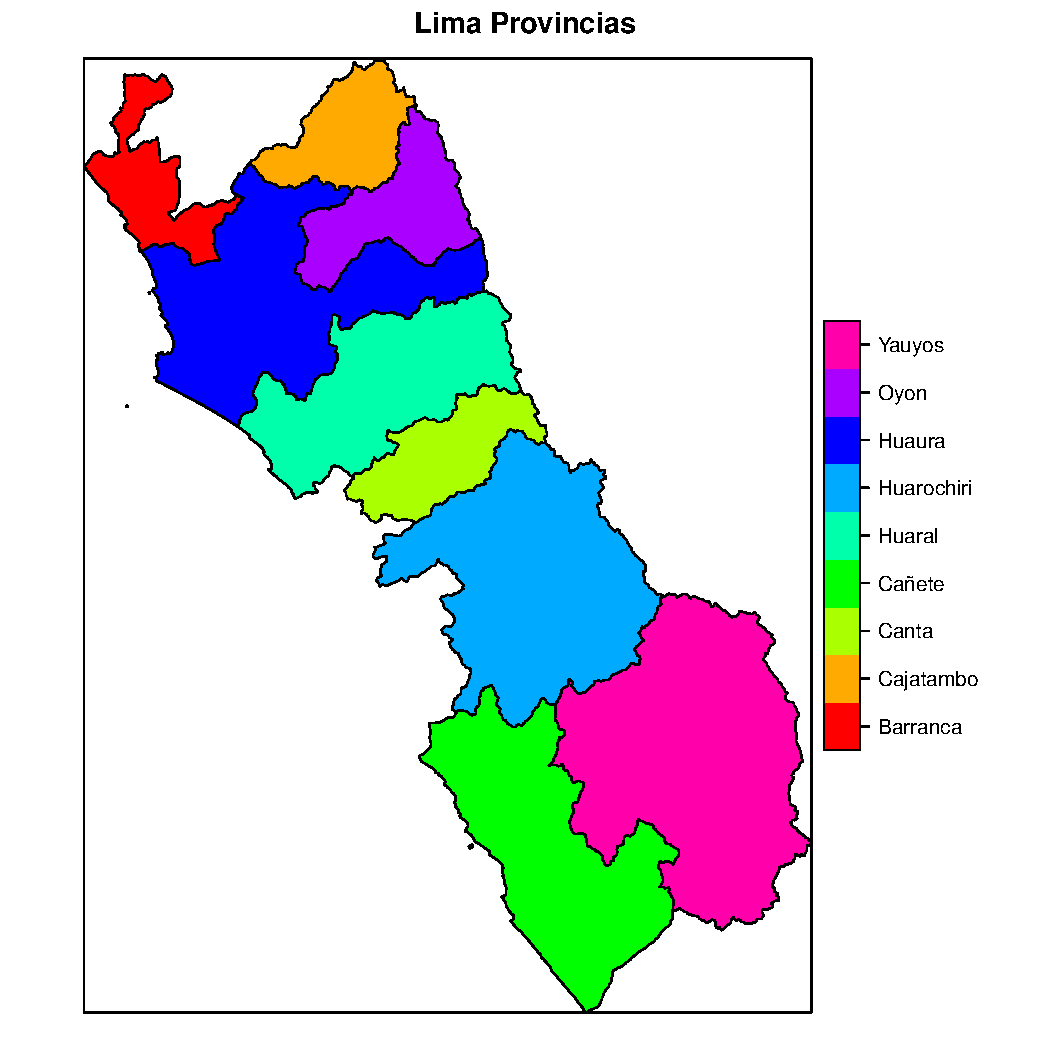
\includegraphics[width=\maxwidth]{figure/unnamed-chunk-4-1} 

\end{knitrout}



\begin{knitrout}
\definecolor{shadecolor}{rgb}{0.969, 0.969, 0.969}\color{fgcolor}\begin{kframe}
\begin{alltt}
\hlcom{#EJEMPLO 4: Se muestra mapa de El Salvador y se selecciona}
\hlcom{#el departamento de Santa Ana}
\hlkwd{library}\hlstd{(sp)}
\hlkwd{library}\hlstd{(maptools)}
\hlkwd{library}\hlstd{(maps)}
\hlstd{SLV}\hlkwb{<-}\hlkwd{readShapeSpatial}\hlstd{(}\hlstr{"SLV_adm1.shp"}\hlstd{,}\hlkwc{proj4string}\hlstd{=}\hlkwd{CRS}\hlstd{(}\hlstr{"+proj=longlat"}\hlstd{))}
\hlkwd{names}\hlstd{(SLV)}
\end{alltt}
\begin{verbatim}
##  [1] "ID_0"      "ISO"       "NAME_0"    "ID_1"      "NAME_1"   
##  [6] "HASC_1"    "CCN_1"     "CCA_1"     "TYPE_1"    "ENGTYPE_1"
## [11] "NL_NAME_1" "VARNAME_1"
\end{verbatim}
\begin{alltt}
\hlstd{SLV}\hlopt{$}\hlstd{NAME_1}
\end{alltt}
\begin{verbatim}
##  [1] Ahuachapán  Cabañas     Chalatenango Cuscatlán   La Libertad 
##  [6] La Paz       La Unión    Morazán     San Miguel   San Salvador
## [11] San Vicente  Santa Ana    Sonsonate    Usulután   
## 14 Levels: Ahuachapán Cabañas Chalatenango Cuscatlán ... Usulután
\end{verbatim}
\begin{alltt}
\hlkwd{plot}\hlstd{(SLV)}
\end{alltt}
\end{kframe}
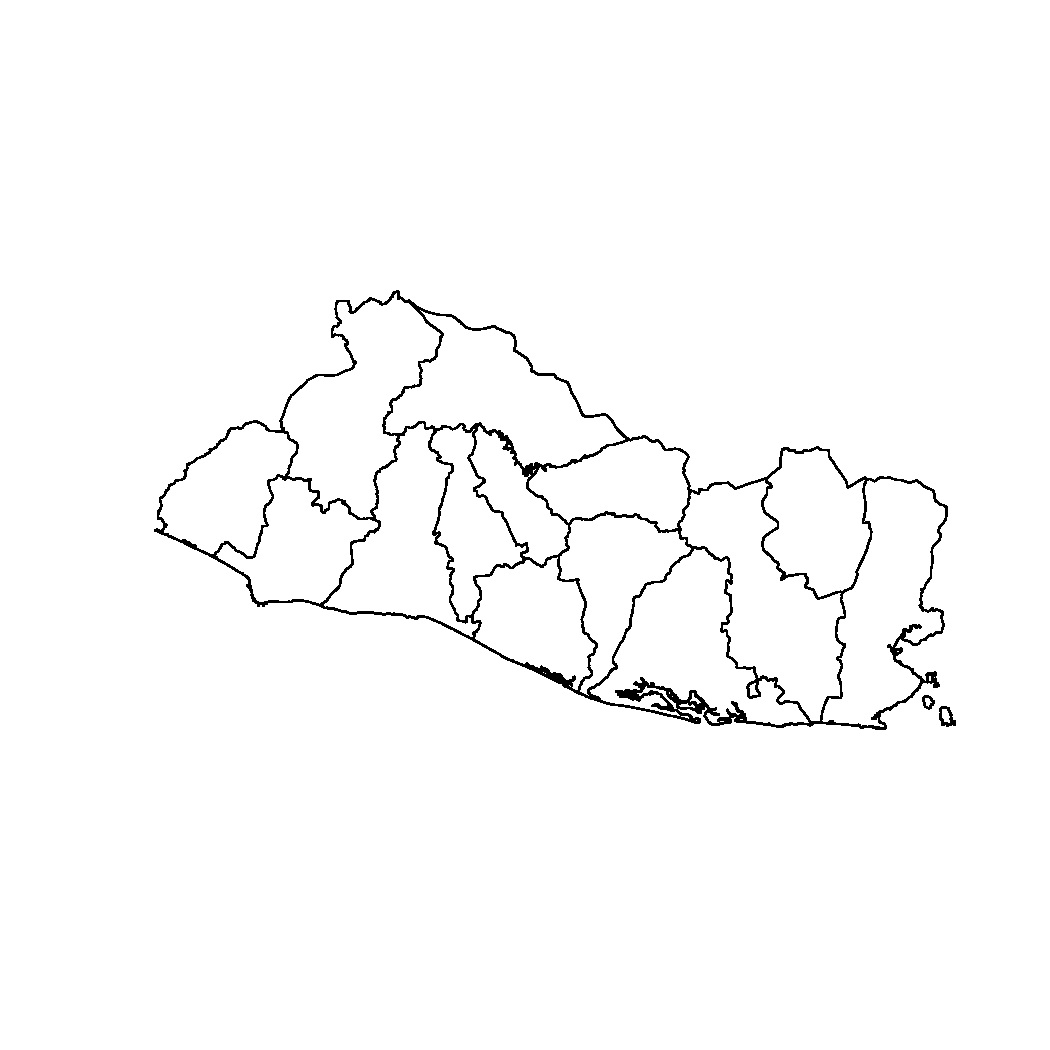
\includegraphics[width=\maxwidth]{figure/unnamed-chunk-5-1} 
\begin{kframe}\begin{alltt}
\hlkwd{plot}\hlstd{(SLV[SLV}\hlopt{$}\hlstd{NAME_1}\hlopt{==}\hlstr{"Santa Ana"}\hlstd{,],}\hlkwc{col}\hlstd{=}\hlstr{"purple"}\hlstd{)}
\hlkwd{title}\hlstd{(}\hlstr{"Santa Ana"}\hlstd{)}
\end{alltt}
\end{kframe}
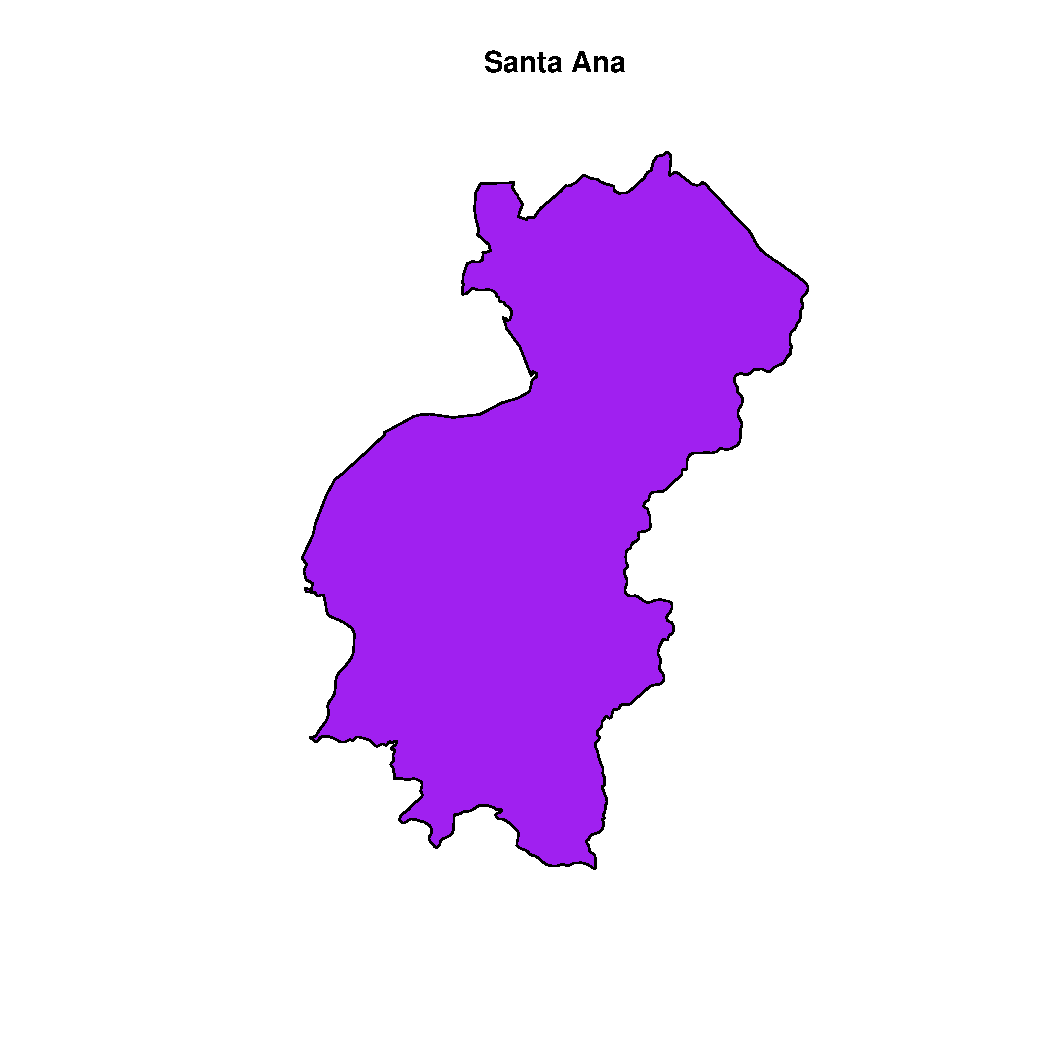
\includegraphics[width=\maxwidth]{figure/unnamed-chunk-5-2} 

\end{knitrout}

\begin{knitrout}
\definecolor{shadecolor}{rgb}{0.969, 0.969, 0.969}\color{fgcolor}\begin{kframe}
\begin{alltt}
\hlcom{#EJEMPLO 5: Departamentos de Francia.}

\hlcom{#Cargamos la libreria maps.}
\hlkwd{library}\hlstd{(maps)}
\hlcom{#Se genera el mapra de francia}
\hlstd{france}\hlkwb{<-}\hlkwd{map}\hlstd{(}\hlkwc{database}\hlstd{=}\hlstr{"france"}\hlstd{)}
\end{alltt}
\end{kframe}
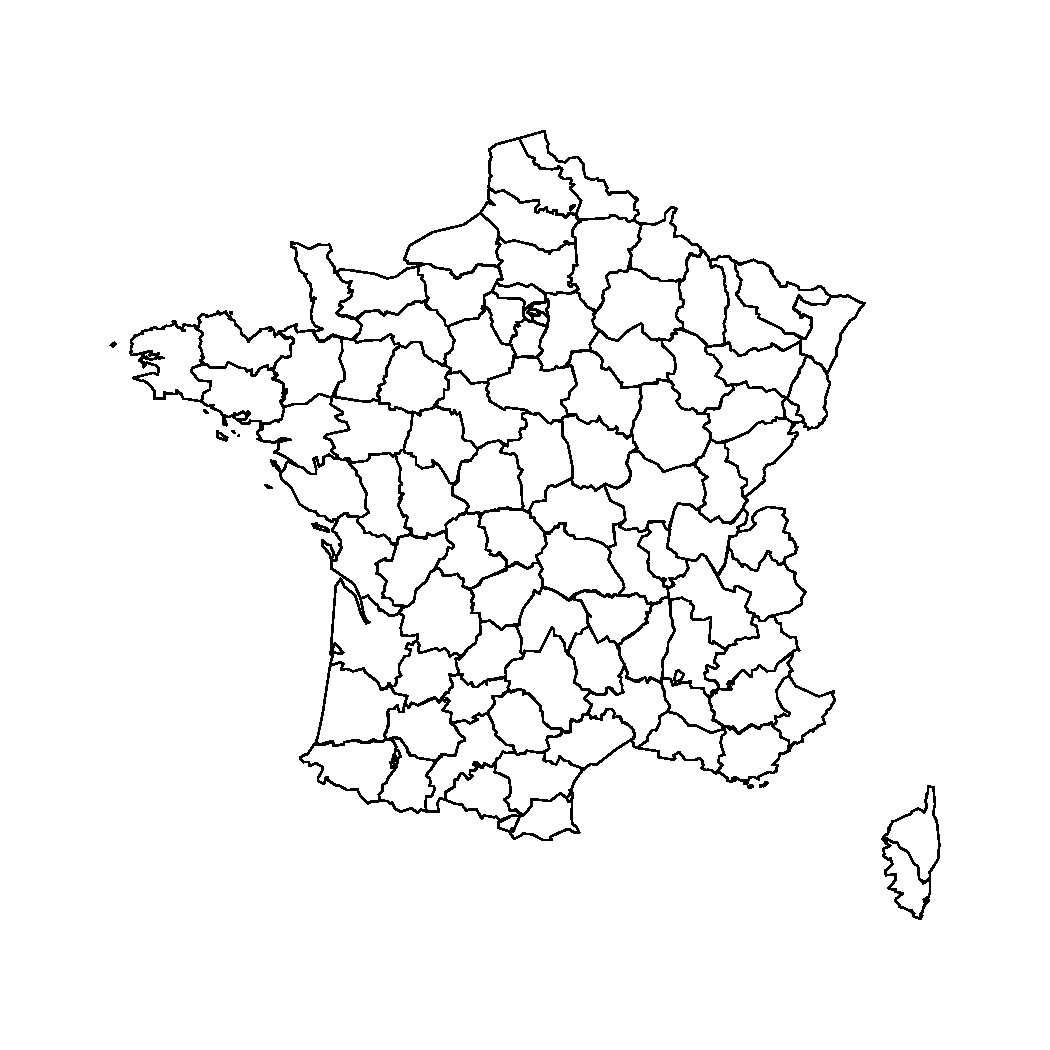
\includegraphics[width=\maxwidth]{figure/unnamed-chunk-6-1} 
\begin{kframe}\begin{alltt}
\hlcom{#Pintamos de color morado "Ain", color azul "Marne", }
\hlcom{#color amarillo "Nord", color rojo "Charente".}
\hlstd{dpt2001}\hlkwb{<-}\hlkwd{c}\hlstd{(}\hlstr{"Ain"}\hlstd{,}\hlstr{"Marne"}\hlstd{,}\hlstr{"Nord"}\hlstd{,}\hlstr{"Charente"}\hlstd{)}
\hlstd{col2001}\hlkwb{<-}\hlkwd{c}\hlstd{(}\hlnum{6}\hlstd{,}\hlnum{4}\hlstd{,}\hlnum{7}\hlstd{,}\hlnum{2}\hlstd{)}
\hlstd{match} \hlkwb{<-} \hlkwd{match.map}\hlstd{(france,dpt2001)}
\hlstd{color} \hlkwb{<-} \hlstd{col2001[match]}
\hlkwd{map}\hlstd{(}\hlkwc{database}\hlstd{=}\hlstr{"france"}\hlstd{,} \hlkwc{fill}\hlstd{=}\hlnum{TRUE}\hlstd{,} \hlkwc{col}\hlstd{=color)}
\end{alltt}
\end{kframe}
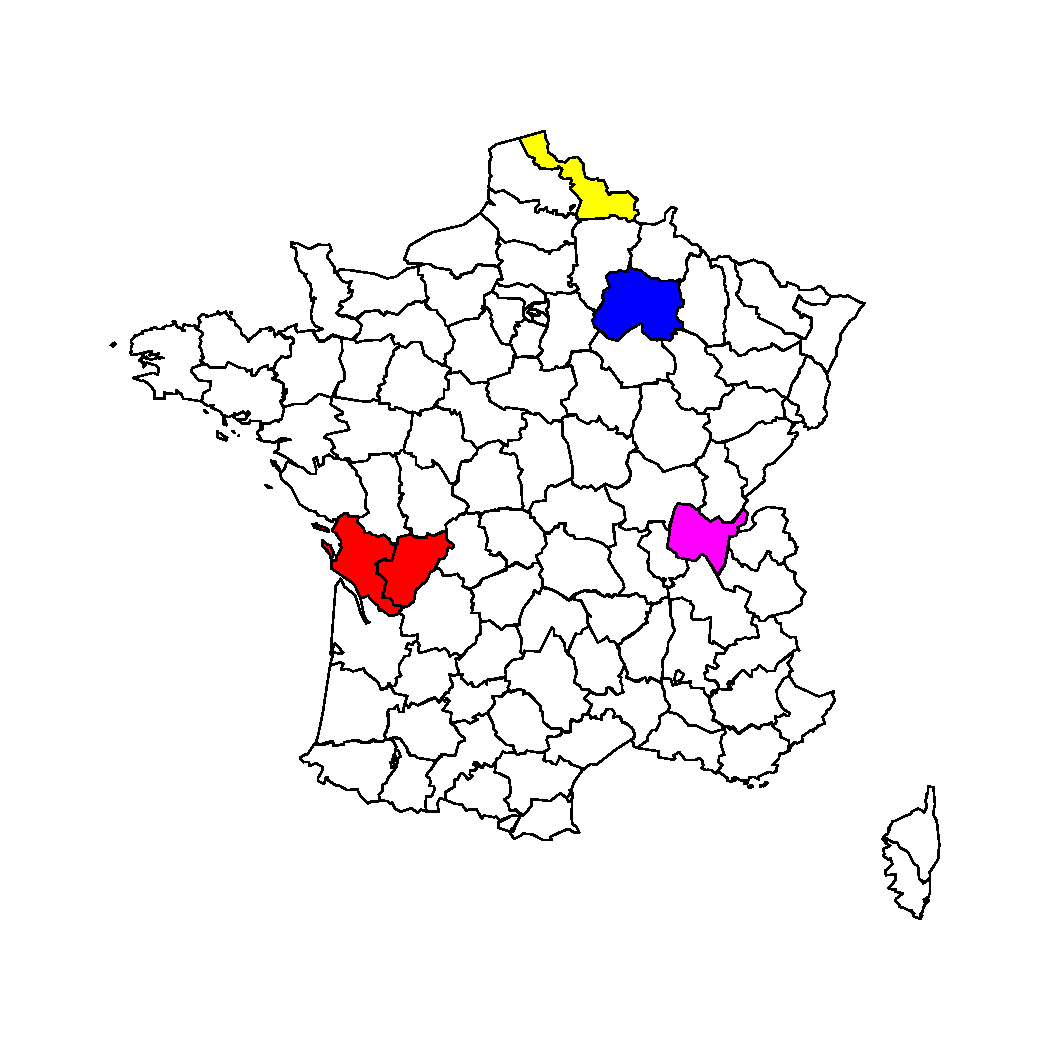
\includegraphics[width=\maxwidth]{figure/unnamed-chunk-6-2} 

\end{knitrout}


\end{document}
